\section{Programas para Controlar a Impressão 3D}
O mundo da Impressão 3D possui um fluxo bem definido:

 
%%%%%%%%%%%%%%%%%%%%%%%%%%%%%%%%%%%%%%%%%%%%%%%%%%%%%%%%%%%%%%%
%
% Welcome to Overleaf --- just edit your LaTeX on the left,
% and we'll compile it for you on the right. If you give
% someone the link to this page, they can edit at the same
% time. See the help menu above for more info. Enjoy!
%
% Note: you can export the pdf to see the result at full
% resolution.
%
%%%%%%%%%%%%%%%%%%%%%%%%%%%%%%%%%%%%%%%%%%%%%%%%%%%%%%%%%%%%%%%
% A bottom-up chart of a TeX workflow
% Author: Stefan Kottwitz
% https://www.packtpub.com/hardware-and-creative/latex-cookbook
\begin{comment}
:Title: A bottom-up chart of a TeX workflow
:Tags: Diagrams;Flowcharts;Smartdiagram;Cookbook
:Author: Stefan Kottwitz
:Slug: smart-priority

A priority chart showing a common TeX workflow
from bottom to top, using the smartdiagram package.
\end{comment}
\begin{adjustbox}{width=\linewidth}
\smartdiagram[flow diagram:horizontal]{Modelagem,
  Fatiamento, Impressão, Acabamento}
\end{adjustbox}



Dado a sua natureza Open Source, que se iniciou nos anos 2000, quando as primeiras
patentes relacionadas a essa tecnologia tiveram seu vencimento, é natural que os
softwares envolvidos neste mundo também tenham seu surgimento ligado a iniciativa Open Source.
Entretanto, alguns dos softwares existentes, não atendem a todas as necessidades
que um usuário de uma Impressora 3D venha a ter, principalmente no que se diz respeito aos Printer Hosts.
Como definido, Printer Host é um software controlador, onde via uma conexão serial,
é possível enviar e receber comandos de uma Impressora 3D. Porém, esta não é sua
principal utilidade, e encontramos Printer Hosts com algumas características que
tem por objetivo dar mais do que o controle da Impressora 3D.

\subsection{Código Livre x Código Proprietário}

\subsection{Exemplos de soluções existentes}

\subsubsection{Repetier Host}
O Repetier Host é um printer host desktop. Além das
ferramentas de controle e gerenciamento da Impressora 3D, ele
possui um ambiente de renderização de objetos 3D, sejam eles
os objetos CAD ou o arquivo GCode, possui monitoração de
temperaturas, e o fatiamento de arquivos CAD para GCode
usando fatiadores externos. Para extender o seu uso, também
existe o Repetier-Server, que permite o controle remoto da
impressora, e o Repetier-Firmware, que pode ser o firmware
embarcado na Impressora 3D. O Repetier Host possuia seu
código aberto até a versão 0.90 lançada em 23 de Junho de
2013 sob a licença Apache, após isso os criadores Marcus
Littwin e Roland Littwin, realizaram um fork e tornaram o
código das versões posteriores proprietário. O projeto
Repetier Host foi desenvolvido usando a tecnologia .Net para Linux e Windows, e
em Objective-C para Mac. O projeto pertence a Hot-World GmbH \& Co. KG, uma empresa dos
irmãos Littwin. A última versão do Repetier Host é a 2.0.5
para Linux e Windows, e 1.0.2 para Mac.
\iffalse
Referências:
- 0.90 codigo: https://github.com/repetier/Repetier-Host
- Licença: https://github.com/repetier/Repetier-Host/blob/master/APACHE-LICENSE-2.0.txt
- Author: https://www.repetier.com/about-us/
- Versão: https://www.repetier.com/download-now/
\fi

\begin{figure}[H]
    \centering
    \caption[Repetier Host]{Visão Geral do Repetier Host}
    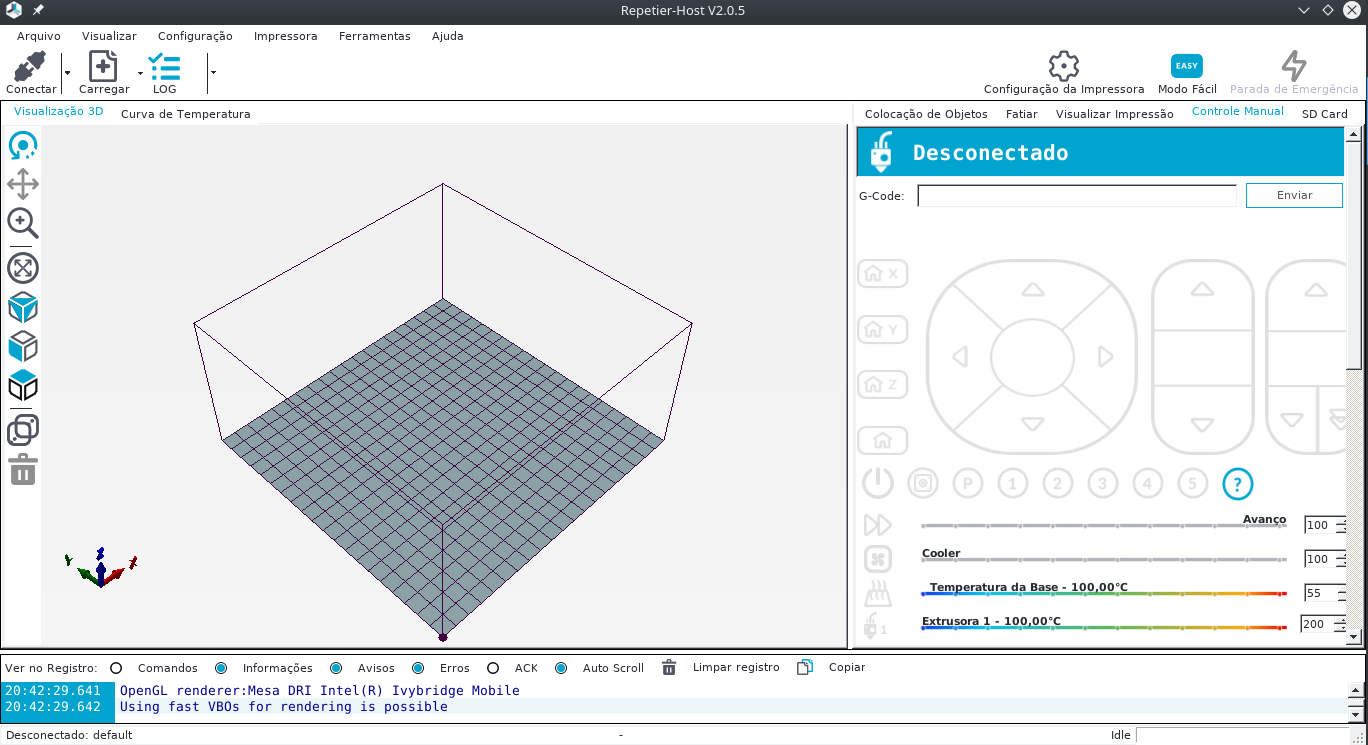
\includegraphics[width=\linewidth]{repetier}
\end{figure}

\subsubsection{OctoPrint}
O OctoPrint é um printer host criado para ser um host remoto, ou seja, ele possibilita
o gerenciamento remoto da Impressora 3D. Ele foi desenvolvido para ser um servidor remoto,
onde o usuário acessa um dispositivo com o OctoPrint instalado, normalmente um RaspberryPi,
e realiza o controle da impressora. Ao conectar a impressora 3D ao RaspberryPi ou
qualquer que seja o dispositivo que esteja servindo o OctoPrint, o usuário tem
acesso a ferramentas como o controle geral da impressora, monitoração de temperaturas,
ser informado através de 'Push Notifications' do status da impressora, além de possuir
 plugins que estendem suas funcionalidades. O OctoPrint possui seu código aberto
 sobre a licença AGPL, e foi criado pela desenvolvedora alemã Gina Häußge. A versão
 1.0.0 do OctoPrint foi lançada em 28 de Outubro de 2013 e nomento da escrita deste trabalho se encontra na versão 1.3.6.
Häußge escreveu o código do OctoPrint usando Python-Flask para a parte servidor, e HTML/JavaScript para o cliente.
\iffalse
Referências:
- Release: https://github.com/foosel/OctoPrint/releases
- Author: https://foosel.net/
- Licença: https://github.com/foosel/OctoPrint/blob/master/LICENSE
- Site: octoprint.org
- Features: https://octoprint.org/#full-remote-control-and-monitoring
https://octoprint.org/#compatible-and-extendable
\fi
\begin{figure}[H]
    \centering
    \caption[Octoprint]{Visão Geral do Octoprint}
    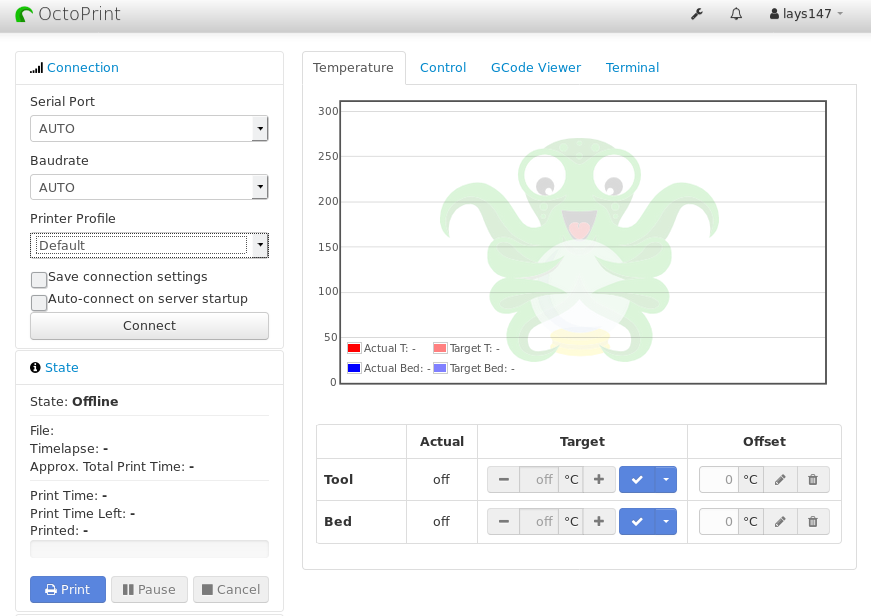
\includegraphics[width=\linewidth]{octoprint}
\end{figure}

\subsubsection{MatterControl}
O Matter Control é um printer host desenvolvido desde 2014 pela empresa MatterHackers sediada
na Califórnia, Estados Unidos. Em suas ferramentas se encontram a renderização do modelo em 3D,
gerenciamento geral da impressora e envios de SMS quando a impressão se conclui.
Possui seu código fonte aberto sobre a licença BSD 2-Clause e é 100\% escrito
com a linguagem de programação C\#. É uma aplicação multiplataforma, porém no ambiente
Linux é limitado as plataformas baseadas em distribuições Ubuntu ou Linux Mint, de acordo com os binários
disponibilizados em seu website. No momento da escrita deste trabalho, o Matter Control se encontra na versão 1.7.5.
\iffalse
Referências:
- Release: https://github.com/MatterHackers/MatterControl/tree/Releases
- Author: Matter Hackers
- Licença: https://github.com/MatterHackers/MatterControl/blob/master/LICENSE
- Site: https://www.matterhackers.com/mattercontrol
\fi

\begin{figure}[H]
    \centering
    \caption[Repetier Host]{Visão Geral do Matter Control}
    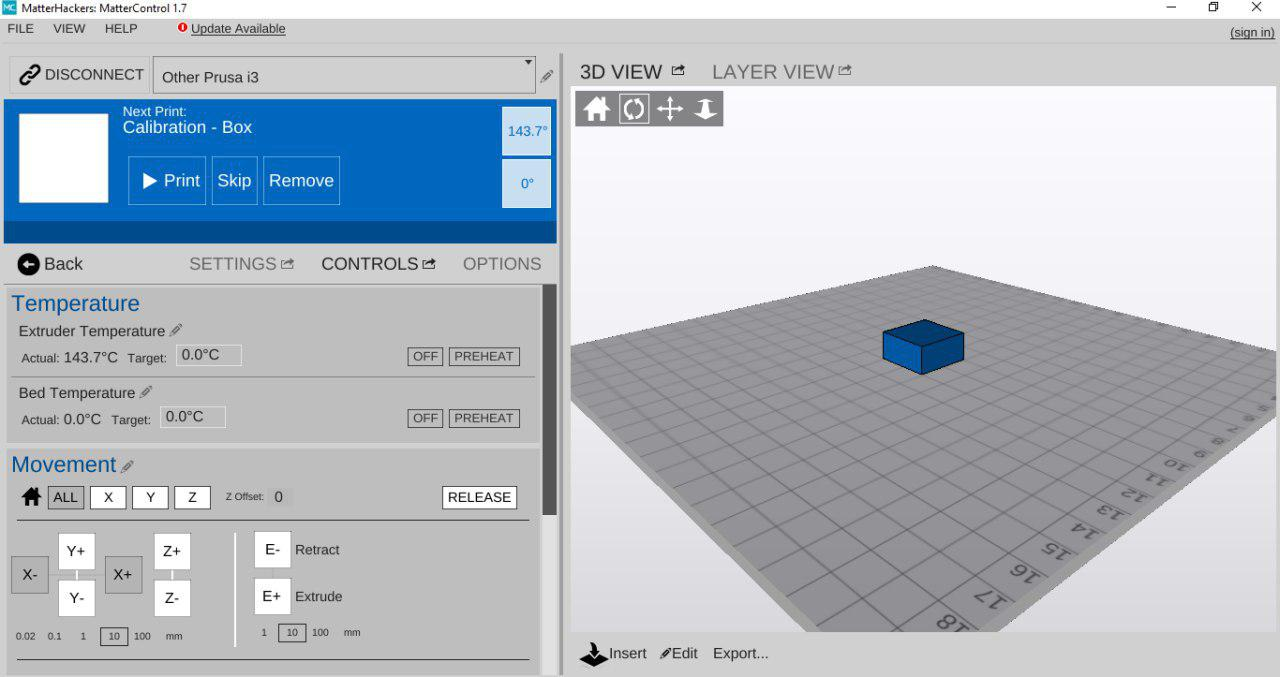
\includegraphics[width=\linewidth]{mattercontrol}
\end{figure}
